\documentclass[12pt]{article}


\usepackage[margin=.8in]{geometry}
\geometry{a4paper} % or letter or a5paper or ... etc
% \geometry{landscape} % rotated page geometry
\usepackage{graphicx}
\usepackage{indentfirst}
\usepackage{wrapfig}
\usepackage[font=small,format=plain,labelfont=bf,up,textfont=it,up]{caption}
\usepackage{listings}
\usepackage[usenames,dvipsnames]{color}
% This is the color used for MATLAB comments below
\definecolor{MyDarkGreen}{rgb}{0.0,0.4,0.0}

% For faster processing, load Matlab syntax for listings
\lstloadlanguages{Matlab}%
\lstset{language=Matlab,                        % Use MATLAB
        frame=single,                           % Single frame around code
        basicstyle=\small\ttfamily,             % Use small true type font
        keywordstyle=[1]\color{Blue}\bf,        % MATLAB functions bold and blue
        keywordstyle=[2]\color{Purple},         % MATLAB function arguments purple
        keywordstyle=[3]\color{Blue}\underbar,  % User functions underlined and blue
        identifierstyle=,                       % Nothing special about identifiers
                                                % Comments small dark green courier
        commentstyle=\usefont{T1}{pcr}{m}{sl}\color{MyDarkGreen}\small,
        stringstyle=\color{Purple},             % Strings are purple
        showstringspaces=false,                 % Don't put marks in string spaces
        tabsize=5,                              % 5 spaces per tab
        %
        %%% Put standard MATLAB functions not included in the default
        %%% language here
        morekeywords={xlim,ylim,var,alpha,factorial,poissrnd,normpdf,normcdf},
        %
        %%% Put MATLAB function parameters here
        morekeywords=[2]{on, off, interp},
        %
        %%% Put user defined functions here
        morekeywords=[3]{FindESS, homework_example},
        %
        morecomment=[l][\color{Blue}]{...},     % Line continuation (...) like blue comment
        numbers=left,                           % Line numbers on left
        firstnumber=1,                          % Line numbers start with line 1
        numberstyle=\tiny\color{Blue},          % Line numbers are blue
        stepnumber=5                            % Line numbers go in steps of 5
        }

% Includes a MATLAB script.
% The first parameter is the label, which also is the name of the script
%   without the .m.
% The second parameter is the optional caption.
\newcommand{\matlabscript}[2]
  {\begin{itemize}\item[]\lstinputlisting[caption=#2,label=#1]{#1.m}\end{itemize}}
  
  \usepackage{graphicx}    % needed for including graphics e.g. EPS, PS
\usepackage{amsmath}	%includes math package
\usepackage{tikz}		%allows for physics graphics
\usepackage{listings}
\usetikzlibrary{scopes}
\usepackage{amssymb}	%includes symbols
\usepackage{cancel}	%used to cancel math texts
\usepackage{gensymb}	%allows for science and engineering symbols
\setcounter{tocdepth}{1}
\DeclareMathOperator{\sech}{sech}
\DeclareMathOperator{\csch}{csch}
\DeclareMathOperator{\dx}{{\it dx}}
\DeclareMathOperator{\dv}{{\it dv}}
\DeclareMathOperator{\du}{{\it du}}

\usepackage{cleveref}%references
\usepackage{paralist}%for compact item
\usepackage[titles]{tocloft}%for table of contents
\usepackage{array}%table with wrapped text
\newcolumntype{L}[1]{>{\raggedright\let\newline\\\arraybackslash\hspace{0pt}}m{#1}}%table with wrapped text


\linespread{1}




% See the ``Article customise'' template for come common customisations

\title{SCUCourses.fish: Course Schedules for Freshman}
\author{Team Aces: James Terry, Nick Peacock, Tracey Acosta, Benjamin Giglione}
\date{\today}

%%% BEGIN DOCUMENT
\begin{document}

\maketitle
\thispagestyle{empty}

\newpage

\thispagestyle{empty}
\renewcommand{\cftsecleader}{\cftdotfill{\cftdotsep}}
\tableofcontents
%\listoftables
\listoffigures
\thispagestyle{empty}

\newpage

\setcounter{page}{1}

\section{Introduction}
All freshmen at SCU goes through an advising period during their summer orientation.  The advising period is brief, stressful, and not as informative as many would like it to be.  Disparities between the number of faculty advisors and students arise frequently.  The first-year schedules themselves are frequently complicated by AP credits, transfer credits, and other exemptions.  Sorting through these exemptions is not a straightforward process, as the number of possible course exemptions is rather large.  Based on AP scores and the math readiness exam a new student could start in four different math courses.  New students, who are unfamiliar with the scheduling process, are told to attempt to determine which courses are covered by their credits and generate schedules before meeting with an advisor.  Their proposed schedules are often poorly constructed, which the advisor must then salvage.  Given that the advising process is relatively brief, advisors cannot always create optimal schedules for students.  The current process leaves many new students without adequate attention, the faculty feeling unhelpful, and the schedules unoptimized.

Team Aces proposes a better solution to SCU's current advising process: SCUCourses.fish, a web application.  On the surface we will have a clean and intuitive interface that will allow new students to input their previously earned credit along with their proposed major.  In turn they will receive optimized first-year schedules outlining which courses they should take.  Our goal is to have the application optimized for the Computer Science and Engineering major and the Web Design and Engineering major.  This web application will include core, C\&I, CTW, and major specific courses.  Students will be asked for their AP scores and possible transfer credits to determine which SCU courses are covered, and will be given possible alternative schedules.  For instance, if a student received an AP score of 5 in Calculus AB his or her schedule will be adjusted so that he or she starts in MATH 13 instead of MATH 11.  The outputted first-year schedules will be exportable in a form that can be easily saved, emailed, and printed.

Using Team Aces' web application will alleviate stress and error caused by this initial advising process.  Students will have a clearer grasp of which courses need to be taken and when they should be taken.  They will also know what information advisors want before their advisement period since the web application will have already asked for it.  Advisors will be able to focus their time on the complex cases that our web application simply cannot handle.  Our application will by no means be perfect, but should be able to handle a majority of cases.  That being said, we believe that our web application will provide a noticeable improvement to the advising process.

\section{Requirements}
The following are the requirements to fit with the needs expressed to our team by the customer. They are split up between functional, non-functional, and constraints.
\subsection{Functional}
The functional requirements are requirements that must be fulfilled in order to make the web application work. The web application will allow students to:
\begin{compactitem}
	\item Work for Computer Engineering and one other engineering major, Web design was choosen
	\item Select any AP and IB tests taken and receive scores
	\item Select courses believed to be covered by transfer credits
	\item Generate a first-year course schedule
	\item Print a proposed schedule

\end{compactitem}

\subsection{Non-functional}
The nonfunctional requirements are requirements describe how the system will behave. The web application will be:
\begin{compactitem}
	\item Portable (will work on major browsers like Internet Explore, Chrome, Firefox, and Safari)
	\item User friendly (straight forward, simplistic, easily understood)


\end{compactitem}

\subsection{Constraints}
The web application must be able to:
\begin{compactitem}
	\item run on design center computers
	\item be a web based application
\end{compactitem}

\section{System Model}

Our web application was designed as follows so as to meet our requirements set by the customer. Initially, as seen in \Cref{1} the user will be prompted to selected his or her major and types of tests (AP and IB) he or she has taken.
\begin{figure}[h!]
\begin{center}

\includegraphics[width=.8\textwidth]{1.png}
\caption{Mock up for major and test selection}
\end{center}
\label{1}
\end{figure}

The user will then be prompted to select the tests he or she has taken in the past. A list of the user's selected tests will populate below, where the user will be able to select the the scores of these selected tests. The user will also be prompted to input his or her Calculus Readiness Exam score if applicable. This can be seen in \Cref{2}.
\begin{figure}[h!]
\begin{center}
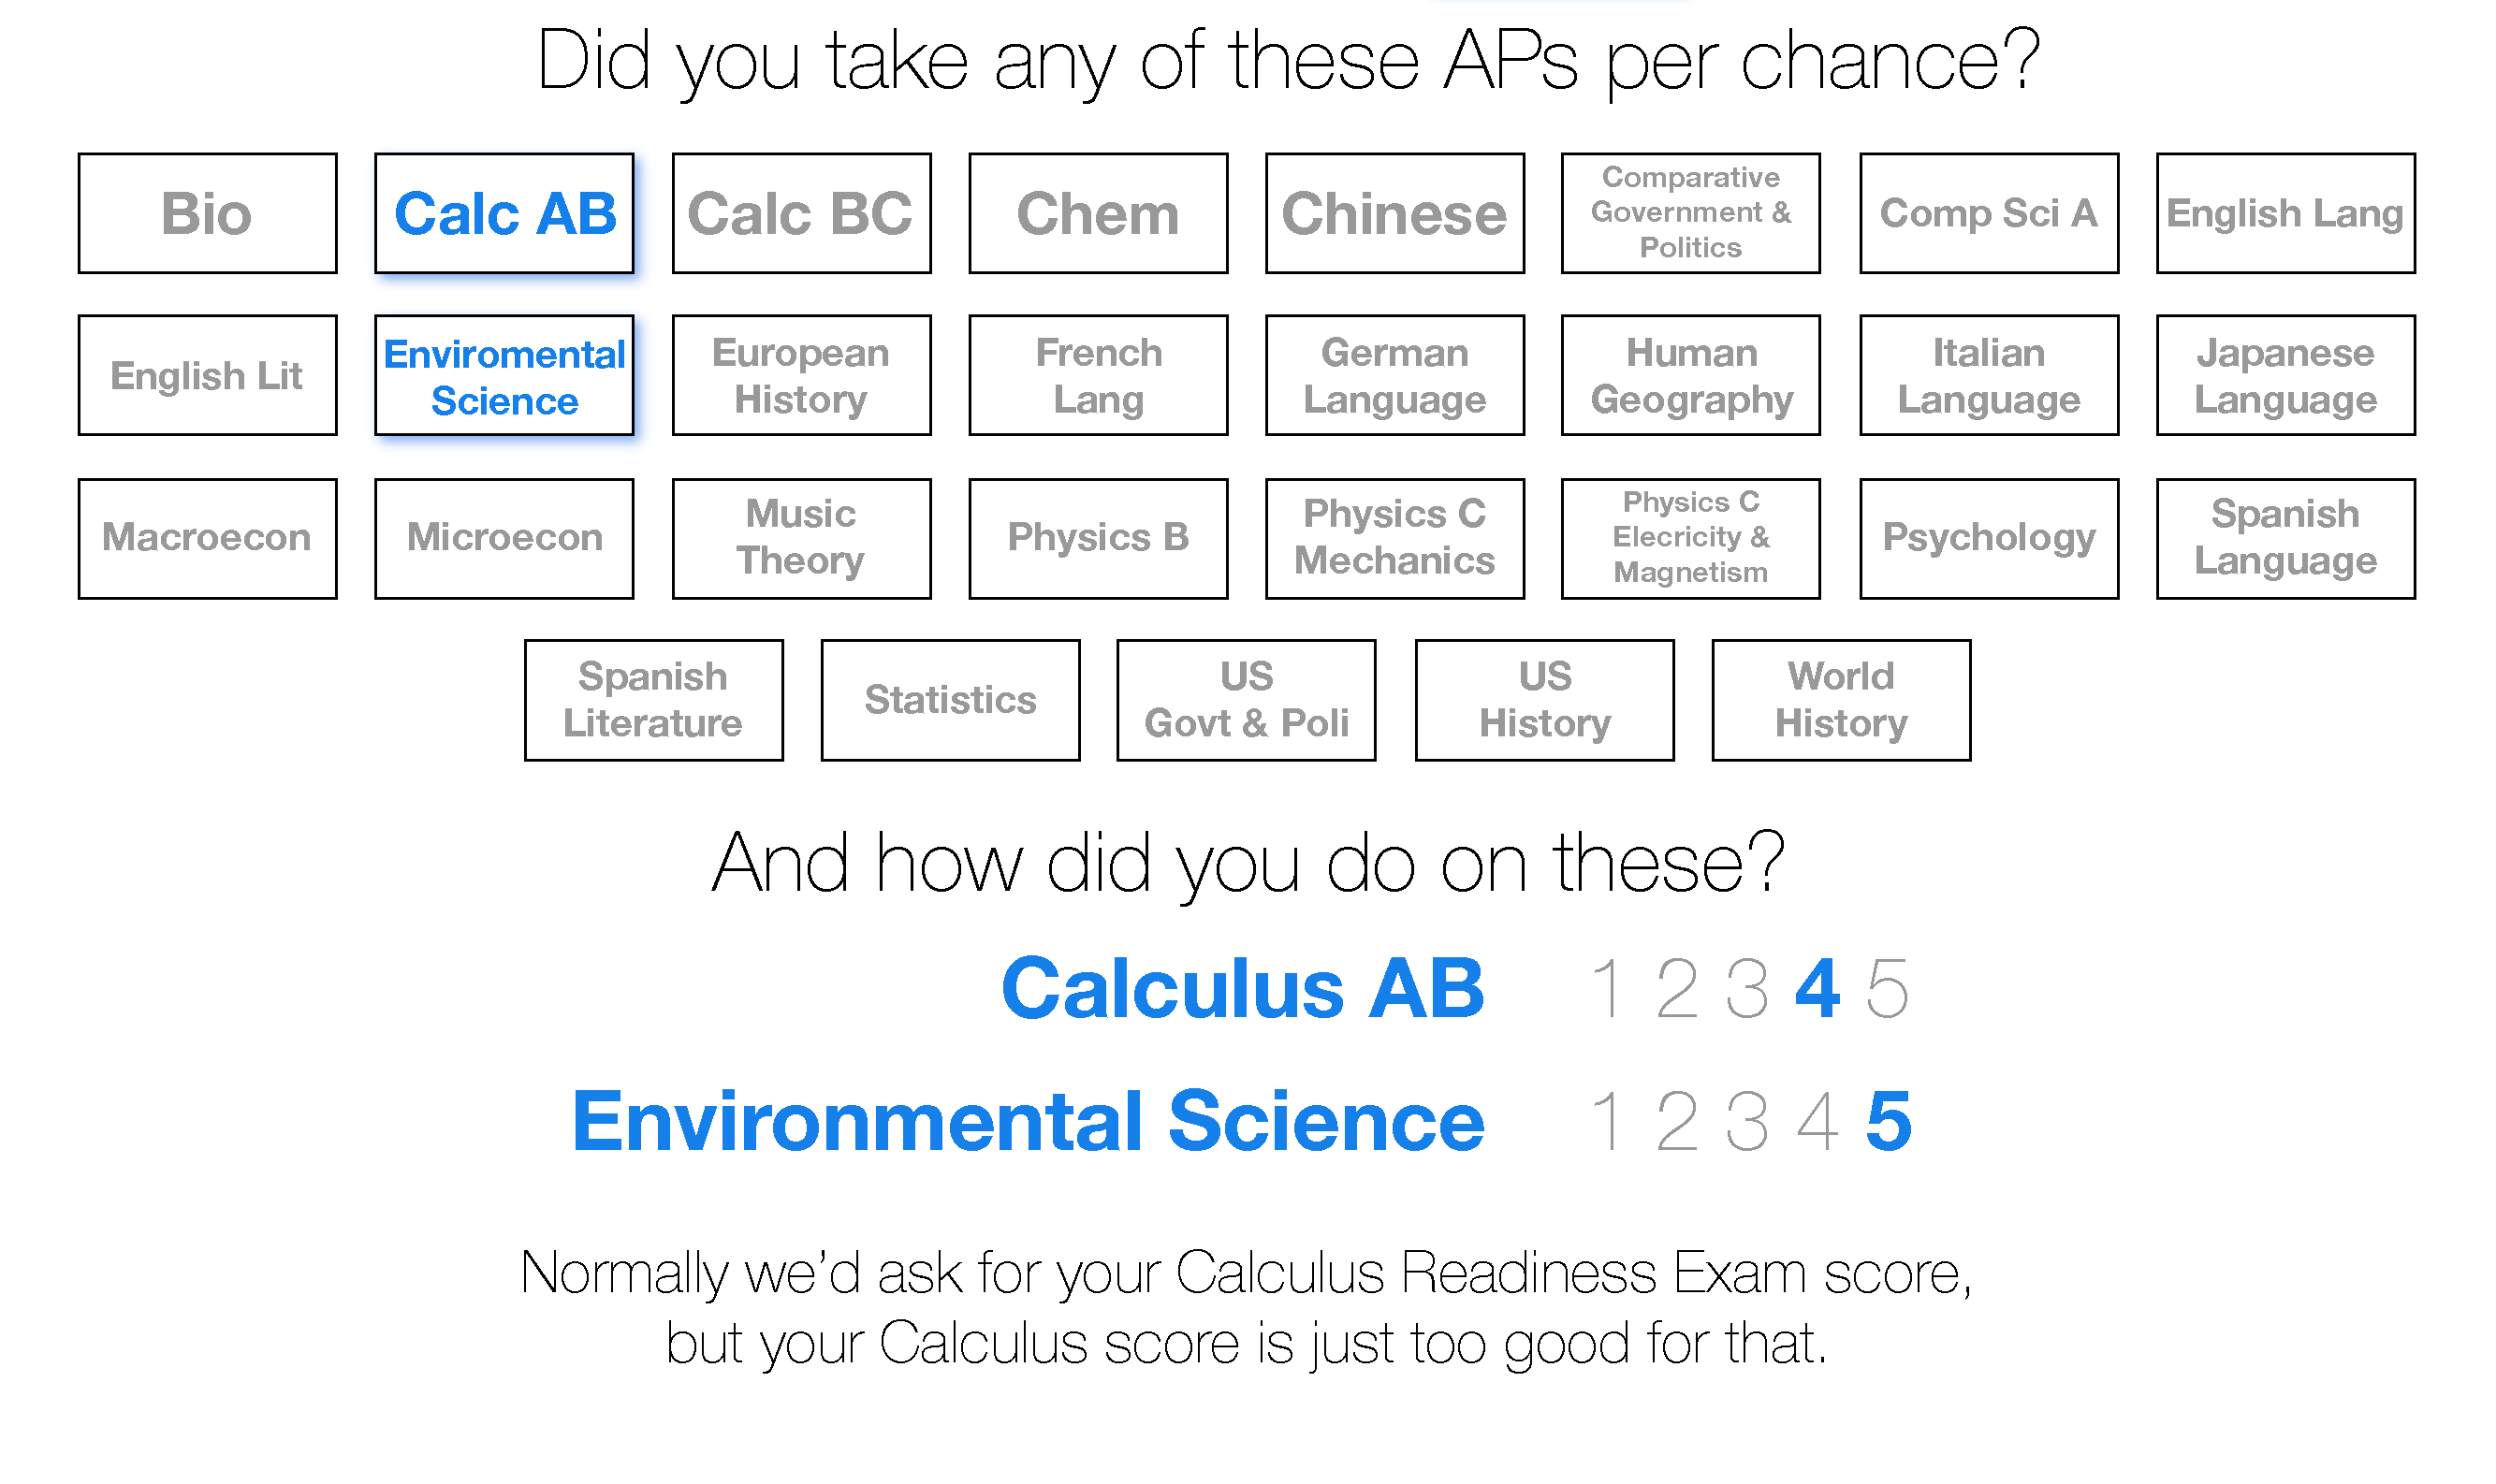
\includegraphics[width=.8\textwidth]{2.png}
\caption{Mock up for entering test scores}
\end{center}
\label{2}
\end{figure}

As \Cref{3} shows, the student will then be prompted to select which courses they have transfer credits for. In the case where they have credit for multiple courses in a series the system will check and cross out the pervious courses in the sequence.

\begin{figure}[h!]
\begin{center}
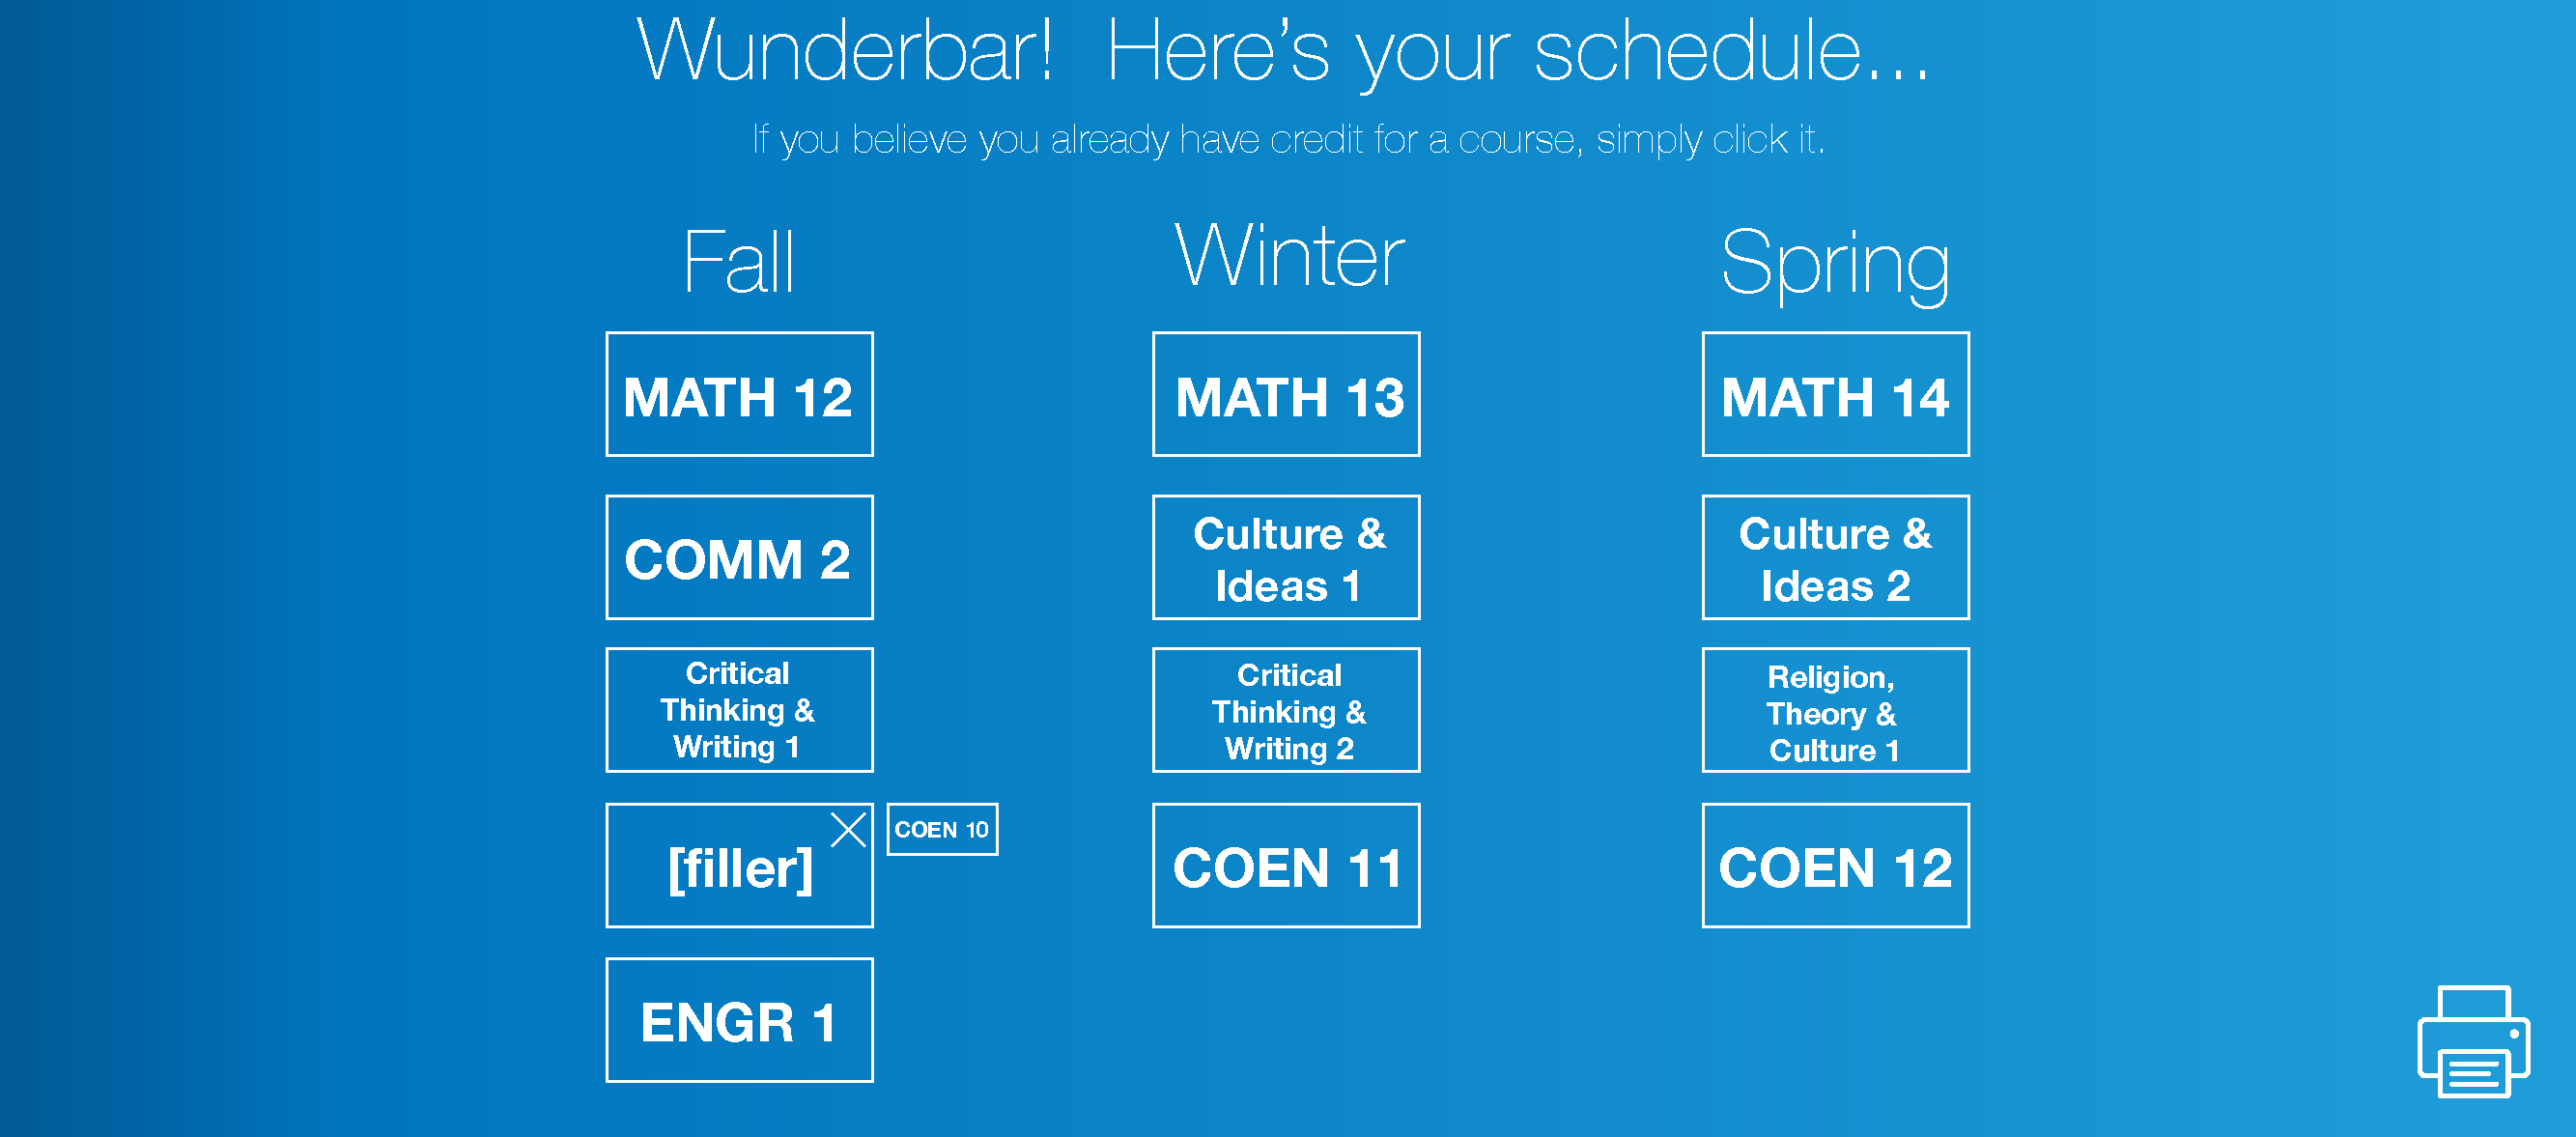
\includegraphics[width=.8\textwidth]{3.png}
\caption{Mock up for entering transfer credits}
\end{center}
\label{3}
\end{figure}

As seen in \Cref{4}, the user will then be shown his or her potential schedule as well as suggesting which CORE credits should be taken in free spots in the schedule. 
\begin{figure}[h!]
\begin{center}
\includegraphics[width=.8\textwidth]{4.png}
\caption{Mock up for potential course schedule}
\end{center}
\label{4}
\end{figure}

The printer version of the schedule can be seen in \Cref{print}. It has a printer friendly color scheme as well as providing an audit of the information the student inputted into the system.
\begin{figure}[h!]
\begin{center}
\includegraphics[width=.8\textwidth]{print.png}
\caption{Mock up for printer friendly schedule}
\end{center}
\label{print}
\end{figure}



\section{Use Cases}

The following use case scenario provides a brief but in-depth explanation of the web application functions and how a user would interact with them.  \Cref{Use} is the use case diagram, which illustrates how the web application work.  The student (user) has the ability to choose his or her major, select any previously taken tests and add the respective scores, select courses that are covered by any previous credit, and view and print the proposed schedule.

Below is an in-depth description of the use case scenarios shown above.\\
Actor: Student\\
Goal: Select major\\
Pre-condition: Actor is a new student at Santa Clara University\\
Post-condition: Schedule adjusts\\
Scenario:
\begin{compactitem}
	\item Click on major drop down list
	\item Click on major
\end{compactitem}
Actor: Student\\
Goal: Input test scores\\
Pre-condition: Actor is a new student at Santa Clara University and chosen a major\\
Post-condition: Actor has successfully inputed test scores and viewed an optimized schedule\\
Scenario:
\begin{compactitem}
	\item Click on types of test
	\item Click on tests taken
	\item Click on scores for tests taken
\end{compactitem}
Actor: Student\\
Goal: Select courses already covered by credit and view optimized schedule\\
Pre-condition: Actor is a new student at Santa Clara University and chosen a major\\
Post-condition: Schedule adjusts\\
Scenario:
\begin{compactitem}
	\item Click on courses already covered
\end{compactitem}
Actor: Student\\
Goal: View and print schedule\\
Pre-condition: Student inputs Credits\\
Post-condition: Schedule Printed\\
Scenario:
\begin{compactitem}
	\item Click print
\end{compactitem}

\begin{figure}[h!]
\begin{center}
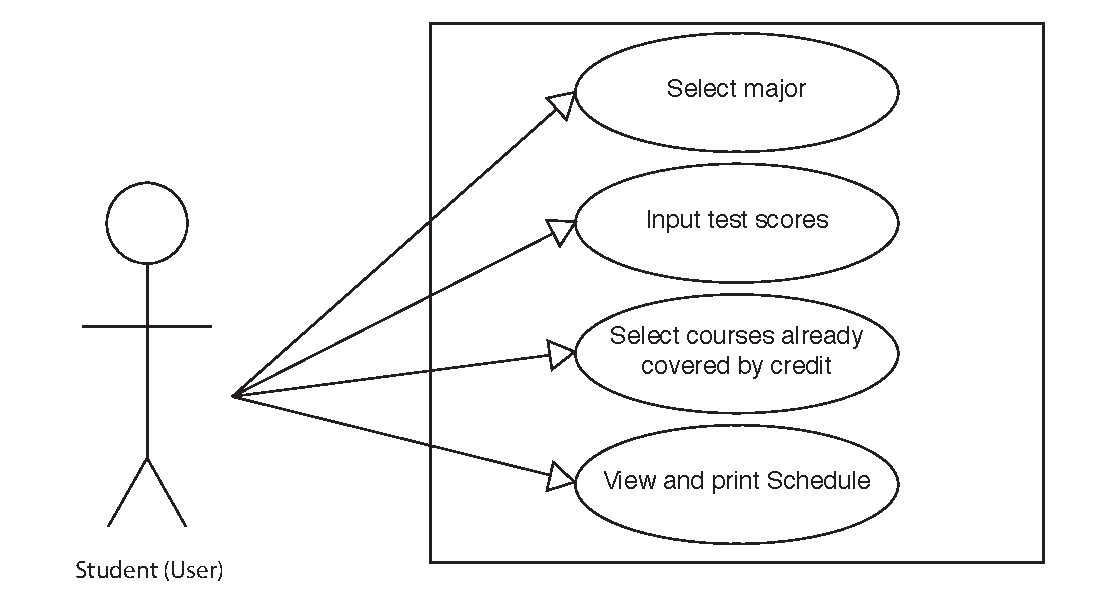
\includegraphics[width=.85\textwidth]{UseCase.pdf}
\caption{Use Case diagram for our system}
\end{center}
\label{Use}
\end{figure}


\section{Architectural Diagram}

SCUCourses.fish will be an online application and users will be able to access our application through any of the major web browsers. The architectural diagram for the application is shown in \Cref{Arch}. The user will log onto the internet using a web browser and navigate to SCUCourses.fish, and it will then pull our information from the servers in order to provide the user with our service. 

\begin{figure}[h!]
\begin{center}
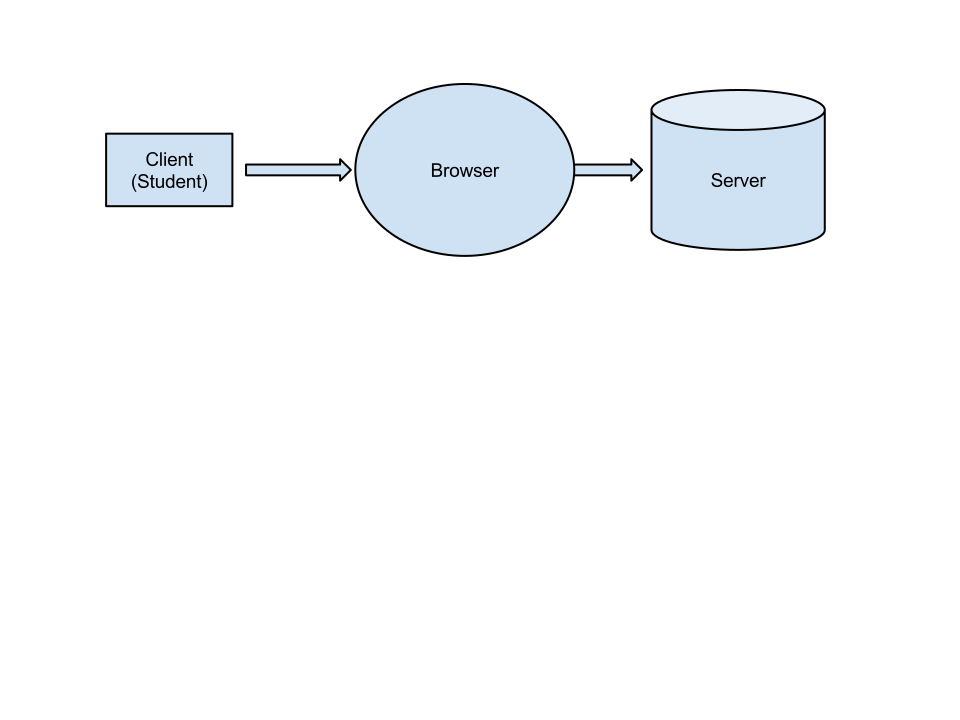
\includegraphics[width=.8\textwidth]{ArchDiag.png}
\caption{Architectural Diagram for our product}
\end{center}
\label{Arch}
\end{figure}

\section{Technologies Used}

To best fulfill the requirements detailed in Section 2 and meet the design shown in Section 3, we will use the following technologies:
\begin{compactitem}
	\item We will be using HTML5 to create the framework for the web application.  HTML stands for HyperText Markup Language and is the most common language for web content.  It provides the structure upon which other code is built on.
	\item We will use CSS3 to format and style the content on the page.  CSS stands for Cascading Style Sheets, and will allow for the stylization of the content so that the web application will look usable.
	\item We will use JavaScript to create the logic upon which the web application runs.  JavaScript is the backbone of the project as the functions created using JavaScript will define the schedules.
	\item This web application will be hosted on the Santa Clara University Design Center servers.
\end{compactitem}

\section{Design Rationale}
For this project we will be working with HTML5, CSS3, and JavaScript.  We chose HTML5 because it is the standard for the web.  It is easily scalable from desktop to mobile devices when paired with CSS3.

CSS3 goes hand in hand with HTML5.  It allows us to create an attractive facade for the structure laid by HTML5.  It is vital that this web application looks appealing as users are put off by old fashioned and ugly design.

We will also use JavaScript for the logic in our web application.  This includes assigning the proper courses to the corresponding variables in HTML5.  It will contain the algorithms the web application uses to generate the student's optimized schedule.  We chose JavaScript because it is fairly easy to use and integrate into HTML5 and CSS3.

We chose to ask students for their AP and IB scores as opposed to what class they are coming from because we do not know which courses will cause exemption.  We give the students the option to select courses from the generated courses that they believe they have credit for.

We chose to use a minimalistic user interface so that users would not be distracted by any unnecessary design.  The ``top to bottom'' flow of the interface follows the natural reading progression.  The limited use of bolding and color draws the user�s attention to the most important sections. 

\section{Risks Table}

This project does come with risks.  To mitigate the damage, we created a risk table detailing the severity, impact, probability and mitigation strategies.    Probability is measured from $0 < p < 1$ with 1 being the most probable.  Severity is measured from 1 to 10, with 10 being the most severe.  The impact these risks have on the project is calculated by multiplying probability with risk.  The risk table is shown in \Cref{Risk}. Throughout the project we had to make adjustments to the risk table, including adding a new risk. One of the minor changes we made was we raised the probability of having bugs and errors from .7 to 1 because we realized it is impossible to write perfect code the first time and we had a few bugs and errors when we wrote our code. The second minor change is we raised the probability of our knowledge of web languages being a risk from .1 to .9 because we only have one Web Design major in our group and the rest of us had to do more research on how to do certain things in JavaScript. The major change we made was adding the risk of misunderstanding the requirements, because during our conversations with the customer and our demo we realized we had made assumptions. 


\begin{table}[h!]
\begin{center}
\begin{tabular}{| L{2cm} | L{2.5cm} | L{1cm} | L{1.5cm} | {2cm} | L{3cm} | L{3cm} | }
\hline

Risk & Consequences & Prob. & Severity & Impact & Mitigations & Mitigations 2\\\hline

Misunderstanding Requirements & Have to redo previously completed work to fit requirements & 0.9 & 10 & 9 & Frequently ask the customer and manager questions clarifying requirements & Demo system to customer and manager before deadline to verify the requirements are met\\\hline

Personnel & Work for that person�s assigned section of the project falls behind & 0.5 & 8 & 4 & Get a significant amount of the work done ahead of time to compensate for possible losses in personnel & Keep a list of understudies so we can re-assign sections to currently active members\\\hline

Time runs out & Not all desired functions of the project completed by the turn-in date & 0.3 & 9 & 2.7 & Prioritize  features in the system and do the most essential first & Perform extensive time management throughout the course of production\\\hline

Bugs and Errors & We�ll have to go back into the code, find out what's causing the problems, and bugfix them & 1 & 2 & 2 & Do ample testing every step of the way to find bugs sooner & Run the program through debugging software\\\hline

Knowledge of web languages & Progress on coding is greatly slowed & 0.9 & 2 & 1.8 & Model our code after some appropriate pre-existing examples of the language & Redistribute coding duties that may be difficult for one or more group members\\\hline

Version control & Entire pages of code must be rewritten & 0.05 & 5 & 0.25 & Use GitHub which has built in Version Control & Divide the code up into multiple documents, to minimize individual risk\\\hline

\end{tabular}
\end{center}
\caption{Possible risks to completing the project}
\label{Risk}
\end{table}

\section{Test Plan}

In order to determine the success of the project, we have devised a series of tests so that the implementation of the web application goes according to plan.  Below are the details of the tests.
\begin{compactitem}
	\item Major Selection
	\begin{compactitem}
		\item Test: User should be able to select Computer Science and Engineering or Web Design and Engineering
		\item Result: Should build major appropriate freshman schedule
	\end{compactitem}
	\item No AP or Transfer credits
	\begin{compactitem}
		\item Test: Enter in no AP scores or scores that are too low and no transfer credits
		\item Result: Should produce default freshman schedule
	 \end{compactitem}
	\item Exempting math
	\begin{compactitem}
		\item Test: Enter AP scores that will exempt each level of Math
		\item Result: Should move up math Curriculum by quarters equal to math courses exempt
	\end{compactitem}
	\item Exempting COEN 10 or science Sequence
	\begin{compactitem}
		\item Test: Enter AP Scores or Transfer Credits for each of the COEN 10 and Science Sequence
		\item Result: Should create a space in schedule filled with CORE
	\end{compactitem}
	\item A space in two quarters in row
	\begin{compactitem}
		\item Test: Enter AP scores or Transfer credits that causes a CORE space two quarters in a row
		\item Result: Should fill with C\&I sequence if the sequence is not already in the schedule otherwise fill with CORE 
	\end{compactitem}
	\item Print
	\begin{compactitem}
		\item Test: Try to print created schedule
		\item Result: Should print created schedule
	\end{compactitem}
\end{compactitem}

The results of our latest tests are that all the functionalities work and we get the desired output for all of our test cases. During our early stages of testing we discovered minor bugs in our code, once those were fixed we began testing the functionalities on our prototype that had end to end functionality. We found a couple of bugs with our Cultures \& Ideas placement, it would fill any two consecutive core sections with C\&I making it possible for it to appear multiple times in a schedule. The second bug is that after the C\&I is placed, if the course where the first C\&I was placed was added back in, it would remove the C\&I 1 but it would leave C\&I 2 in the schedule by itself.Our solution to these bugs was to delete the C\&I placement after every change and add it back in if there were still two consecutive core courses. What we noticed was that our solution not only fixed our bugs but also optimized the placement of the C\&I courses by making sure it is placed in the earliest possible slot. 


\section{Development Timeline}

In order to make sure we stay on track and finish the application on time we have a Gantt chart, shown in \Cref{Gantt}.  The Gantt chart shows the assignments that need to be completed, the person who is in charge of completing it and the deadline for that assignment. 

\begin{figure}[t!]
\begin{center}
\includegraphics[width=1.5\textwidth, angle =90]{Gant.png}
\caption{GANTT chart for the development of our team project}
\end{center}
\label{Gantt}
\end{figure}

\section{Lessons Learned}

While working on the project and presenting it, we learned a couple of lessons. The three most significant lessons we learned were presentation etiquette, not to use prezi, and to talk and demo to our customer frequently. When we presented our design review, we learned about presentation etiquette through mistakes that we made. We now know that we should wear appropriate dress shoes, we should not stand in front of the screen nor turn or back to the audience, and we should not make any motions with our phone in our hand. During that presentation, we presented using prezi. We now know that we should not use prezi for professional presentations because they can be distracting and there are very few opportunities to use it correctly. Lastly we learned to talk and demo to our customer frequently because when we had our first demo, our customer pointed out to us some of the assumptions we made and we were able to clear up any misunderstandings of the requirements. The lesson is that if you meet with the customer earlier and more frequently, you will make sure you understood the requirements and you have a greater chance of delivering what the customer wants. 

\pagebreak
\appendix


\section{User Manual}

The first step that you will take is to log onto a web browser in order to open our application. If you are using a Mac you will need to open Safari or Firefox, if you are using Windows you will need to open Internet Explorer or Firefox. Once the web browser is open, type in the url ``scucourses.fish'', this will open up our application.

Now you are ready to create your schedule. You need to select between the Computer Engineering (COEN) major or the Web Design and Engineering major to begin generating a schedule. There is a standard schedule that has been created at the bottom of the page, from this point on you have the ability to view the schedule, and it will update and become customized with each question you answer. A question will appear, under the previous question, about how certain you are about your major, select ``Fairly Confident'' or ``Double Plus Unconfident''. Next another question appears, if you have any experience with C programming you can select ``Oh, yeah'', and if you have no experience select ``I know that I know nothing''. 

Now you are presented with the option to enter AP or IB credit. If you took any AP exams select the ``AP'' button, it will now show you a list of exams. Select any of the exams you took, and upon selection click on what your score is. If you took any IB exams select the ``IB'' button, it will now show you a list of exams. Select any of the exams you took, and upon selection click on what your score is. If you tested out of any calculus class you will see a line below the test scores that reads ``You placed out of the calculus readiness exam. Nerd.'', move on to the next question. If you did not place out of calculus there will be a question asking you if you passed the calculus readiness exam so select your answer based on your score. The next question asks if you have any transfer credit. If you do not have any transfer credit then you are done with your schedule. If you do have transfer credit, select the areas in which you have credit, and then select the courses you have credit for. Now you are done customizing your schedule. 
If at any time you make a mistake you are able either unselect a button by clicking on it again or you may simply click on the correct button. If you make several mistakes, or chose to start over, you make click on the word ``Reset'' on the top right corner and it will reset everything. When you are done customizing your schedule, you may print it out a printer friendly version of your schedule by clicking on the printer icon at the bottom left corner of the page. 






\end{document}